\chapter{World Model as Planner}
\label{chap:wm-planner}

\section{Motivation}

The previous chapter defined the risks of treating a world model as a full training-time environment: compounding error, off-manifold transitions, and value corruption. This does not imply that the model is useless for decision-making. Short-horizon predictions may still be accurate enough to improve action selection at inference time, even if they are not reliable enough to support full online training.
This chapter explores that idea. Instead of using the world model to generate training data, we use it only to expand the agent's decision process at test time. The key idea is simple: the policy proposes several candidate actions, the world model simulates their short-term consequences, and the offline-trained critic selects the most promising outcome. Crucially, no parameters are updated during this process; the world model is used purely as a predictive rollout mechanism, and the critic remains the sole learning-derived signal.
The remainder of this chapter defines three inference-time planners:
sampling-based Best-of-$N$ search, gradient-based refinement, and a
flow-matching $Q$-guided update. Their empirical comparison is reported
in \S\ref{sec:exp-mpc}.

% ---------------------------------------------------------------------
% \section{Best-of-$N$ MPC at inference}
\section{Best-of-$N$ Value Guided Planning}
\label{sec:mpc-bon}

The simplest way to use the world model at inference time is to treat it as a proposal evaluator. At a given latent state, we sample multiple candidate action chunks from the trained policy, simulate their consequences for a short horizon using the world model, and then select the candidate that appears best according to the critic.
Concretely, and as illustrated in Figure~\ref{fig:mpc-bon}, $N$ candidate action chunks are drawn from the BC-flow actor at the current latent. Each candidate is then rolled forward for $H$ steps using the world model, where continuation actions are sampled from the policy conditioned on the predicted latents. This produces a short imagined trajectory for each candidate, which is then scored using the critic. The first action chunk of the highest-scoring trajectory is executed in the real environment.

\paragraph{The score $J$.}
To evaluate each candidate action chunk $a_0^{(i)}$, we consider three alternative scoring functions based on the critic and the world model rollout:
\begin{align}
    J_{\text{Q-term}}(a_0^{(i)}) &= Q_\phi(z_H^{(i)}, a_H^{(i)}), \\
    J_{\text{Q-all}}(a_0^{(i)})  &= \sum_{h=0}^{H} Q_\phi(z_h^{(i)}, a_h^{(i)}), \\
    J_{\text{dense+Q}}(a_0^{(i)}) &= -\sum_{h=0}^{H} \|z_h^{(i)} - z_g\|_2 / s
                                  \;+\; Q_\phi(z_H^{(i)}, a_H^{(i)}).
\end{align}
Each variant reflects a different hypothesis about how to best use the critic over imagined trajectories. Q-term evaluates only the terminal state, treating the world model as a short-horizon proposal generator. Q-all aggregates critic values along the full rollout, effectively encouraging trajectories that remain high-value throughout. Dense+Q adds an explicit geometric shaping term in latent space, combining critic-based evaluation with distance-to-goal information.

\paragraph{Proposal sampling and the connection to Q-chunking.}
Candidate action chunks are generated directly from the BC-flow policy. Specifically, we sample noise vectors $x_0^{(i)} \sim \mathcal{N}(0, I_{25})$ and apply $S = 10$ Euler integration steps through the flow model (cf.\ Figure~\ref{fig:fql-bg}) to obtain $N$ structured action chunks. This is equivalent to the best-of-$N$ sampling procedure used in Q-chunking \cite{li2026reinforcementlearningactionchunking}, where multiple candidate action sequences are generated and ranked before execution. The key difference here is that ranking is performed after simulating each candidate through the world model rather than evaluating it only at the current state.

\paragraph{Continuation re-sampling.}
When rolling a candidate forward, we do not execute its actions open-loop. Instead, at each predicted latent state, new continuation actions are sampled from the policy conditioned on that state. This ensures that the imagined trajectory reflects the same closed-loop behaviour the policy would exhibit in the real environment, rather than an unrealistic fixed-action rollout.

\begin{figure}[t]
    \centering
    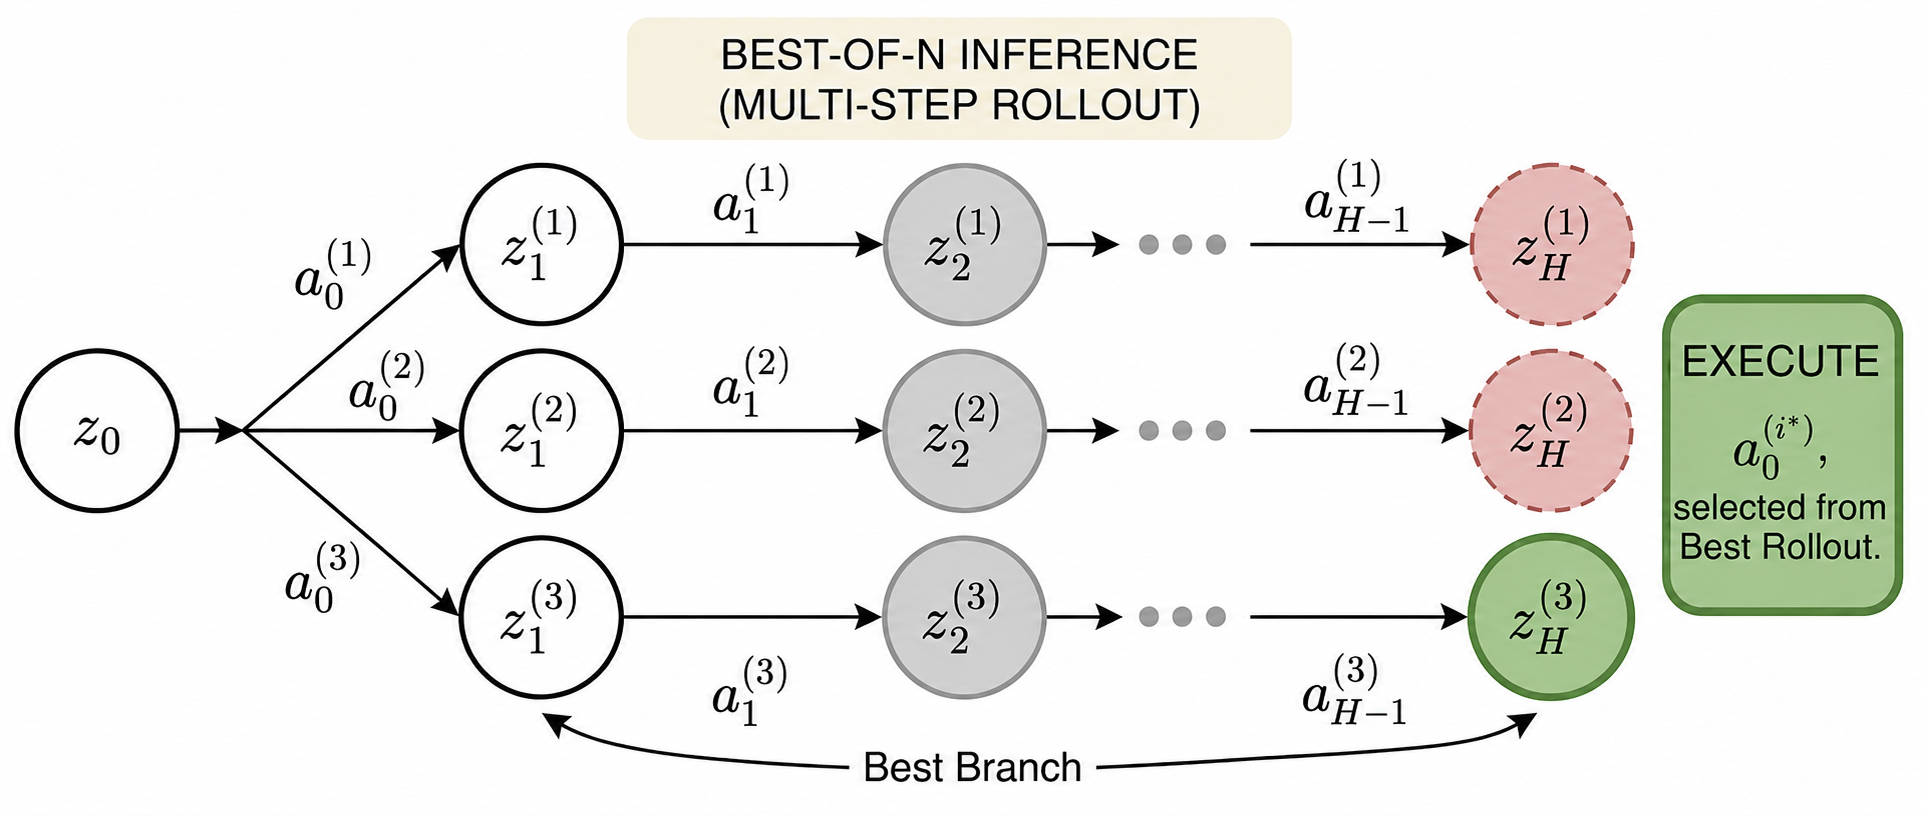
\includegraphics[width=\linewidth]{figures/bon.png}
    \caption{Illustration of Best-of-$N$ MPC at inference time. Starting from the current latent state $z_0$, the policy samples $N$ candidate first action chunks $\{a_0^{(i)}\}_{i=1}^N$. Each candidate defines a separate rollout branch, which is then propagated for $H$ steps through the world model with continuation actions re-sampled on-policy at each predicted latent state. This produces $N$ imagined trajectories with terminal latents $\{z_H^{(i)}\}_{i=1}^N$. Each rollout is scored using the critic-based objective $J$, and the branch with the highest score is selected. Only the \emph{first} action chunk $a_0^{(i^\star)}$ from the best-scoring branch is executed in the real environment.}
    \label{fig:mpc-bon}
\end{figure}

The horizon and scoring-function sweep is reported in
\S\ref{sec:exp-mpc-frozen} (Table~\ref{tab:mpc-bon}). It tests whether
additional model lookahead improves ranking or instead makes the critic
score less reliable because of predictor drift.

\begin{algorithm}[h]
\caption{Best-of-$N$ MPC inference.}
\label{alg:mpc-bon}
\begin{algorithmic}[1]
\Require current latent $z_t$, BC-flow actor $\pi_\theta$, critic $Q_\phi$, world model $f_\psi$, hyperparameters $N$, $H$, scoring $J$.
\State Tile $z_t$ to a batch $z_{\text{batch}} \in \mathbb{R}^{N \times d_z}$.
\State Sample $\{x_0^{(i)}\} \sim \mathcal{N}(0, I_{25})$ and set $a_0^{(i)} \leftarrow \Phi_\theta(z_{\text{batch}}, x_0^{(i)})$.
\State Roll each candidate forward $H$ steps through $f_\psi$ with on-policy continuation re-sampling.
\State Compute score $s_t^{(i)}$ for each candidate using $J$.
\State \Return $a_0^{(i^\star)}$ with $i^\star = \arg\max_i s_t^{(i)}$.
\end{algorithmic}
\end{algorithm}

% ---------------------------------------------------------------------
\section{Gradient-Based Value Guided Planning}
\label{sec:mpc-grad}

Best-of-$N$ MPC is fundamentally limited by the support of the
proposal distribution: it can only select actions that are already
likely under the policy. Since the world model is differentiable, we
can go beyond this limitation by directly optimising the selected
action using gradients through the model.

\paragraph{Update rule.}
Starting from the BoN winner, we run $K$ raw gradient ascent steps,
\begin{equation}
    a_0 \;\leftarrow\; \mathrm{clip}\!\Big(a_0 + \eta\,\nabla_{a_0} J(a_0;\,z_t),\;-1,\;1\Big),
    \qquad k = 1, \dots, K,
    \label{eq:mpc-grad}
\end{equation}
with step size $\eta = 0.01$ and $K=5$. This procedure, referred to
as Grad-MPC, can be seen as replacing discrete sampling in MPC with
continuous optimisation through backpropagation across the world
model rollout. It is closely related to TD-MPC-style refinement \cite{hansen2022temporaldifferencelearningmodel}, but
differs in that the optimisation is performed entirely at inference
time and is applied only to the first action chunk.

\paragraph{Gradient-step sensitivity.}
The number of gradient steps controls the trade-off between refinement
and critic extrapolation. Too few steps provide little movement beyond
the sampled proposal, while too many steps may push actions into regions
where the critic has limited support. The sweep over refinement settings
is reported in \S\ref{sec:exp-mpc-frozen} (Table~\ref{tab:mpc-grad}).

% ---------------------------------------------------------------------
\section{Flow-Matching $Q$-Guided Planning}
\label{sec:mpc-fmq}

Grad-MPC relies on iterative optimisation, which introduces both
computational overhead and sensitivity to step size. Flow Map
$Q$-Guidance (FMQ) \cite{ziakas2026aligningflowmappolicies} replaces this iterative process with a
closed-form update derived from a trust-region approximation of the
critic.

\paragraph{Trust-region objective.}
Let $\pi^{\mathrm{ref}}(\cdot \mid z)$ be a reference flow-map
policy producing actions $a_1 = a_r + (1-r)\,u^{\mathrm{ref}}_{r,1}(a_r \mid z)$
through the two-time average velocity $u^{\mathrm{ref}}_{r,1}$.
We seek a perturbation of this velocity field that improves the
critic while remaining close to the original policy:
\begin{equation}
    \max_{u_{r,1}}\; Q_\phi\!\big(z,\, a_r + (1-r)\, u_{r,1}(a_r \mid z)\big)
    \qquad\text{s.t.}\qquad
    \big\|u_{r,1} - u^{\mathrm{ref}}_{r,1}\big\|_2 \;\le\; \eta.
    \label{eq:mpc-fmq-objective}
\end{equation}

\paragraph{Closed-form solution.}
The solution to this constrained optimisation problem is given by:
\begin{equation}
    \boxed{\;u^{\,*}_{r,1}(a_r \mid z) \;=\; u^{\mathrm{ref}}_{r,1}(a_r \mid z) \;+\; \eta\,\frac{\nabla_a Q_\phi(z, a_1)}{\big\|\nabla_a Q_\phi(z, a_1)\big\|_2}\;.}
    \label{eq:mpc-fmq-target}
\end{equation}
This update has a clear interpretation: it preserves the original
policy direction and adds a fixed-magnitude step in the direction
that most increases the critic.

\paragraph{Inference-time FMQ.}
FMQ replaces the iterative refinement loop of Grad-MPC with a single
application of this update. Otherwise, the proposal sampling,
rollout, and scoring procedure are identical.
Algorithm~\ref{alg:mpc-fmq} shows the complete FMQ inference procedure.
Each policy proposal is refined once using a normalised critic gradient
through the world-model rollout, then the refined proposals are scored
and the best first action chunk is executed.

\begin{algorithm}[h]
\caption{Inference-time FMQ planning.}
\label{alg:mpc-fmq}
\begin{algorithmic}[1]
\Require current latent $z_t$, actor $\pi_\theta$, critic $Q_\phi$, world model $f_\psi$, scoring rule $J$, hyperparameters $N$, $H$, $\eta$.
\State Sample first-action proposals $\{a_0^{(i)}\}_{i=1}^N \sim \pi_\theta(\cdot \mid z_t)$.
\For{$i = 1, \dots, N$}
    \State Roll out $a_0^{(i)}$ for $H$ world-model steps, sampling continuation actions from $\pi_\theta$ with fixed noises.
    \State $g_i \leftarrow \nabla_{a_0^{(i)}} J(\tau_i)$ by backpropagating through the rollout $\tau_i$.
    \State $\tilde a_0^{(i)} \leftarrow \mathrm{clip}\big(a_0^{(i)} + \eta\, g_i / (\|g_i\|_2+\varepsilon),\;-1,\;1\big)$.
\EndFor
\For{$i = 1, \dots, N$}
    \State Roll out $\tilde a_0^{(i)}$ from $z_t$ for $H$ world-model steps with fresh continuation actions from $\pi_\theta$.
    \State $s_i \leftarrow J(\tilde\tau_i)$ for the resulting trajectory $\tilde\tau_i$.
\EndFor
\State \Return $\tilde a_0^{(i^\star)}$ with $i^\star = \arg\max_i s_i$.
\end{algorithmic}
\end{algorithm}

\paragraph{Sensitivity on the base critic.}
FMQ relies on the critic providing a locally meaningful gradient
direction. Since the critic is trained only on offline data generated by
the behaviour policy, large FMQ updates can move actions outside its
support. The trust-region sweep is reported in \S\ref{sec:exp-fmq-base}
(Table~\ref{tab:mpc-fmq-basepolicy}).

\paragraph{FMQ as a training signal.}
FMQ can also be used to generate improved supervision targets.
In the training pipeline of Chapter~\ref{chap:mpc-distillation},
FMQ is used to select action labels, which are then used to train the
actor via standard behavioural cloning in latent space.

% ---------------------------------------------------------------------
\section{Summary}

This chapter defined planners that keep the world model in a
short-horizon proposal role and delegate final action ranking to an
offline-trained critic. Best-of-$N$ search, gradient refinement, and FMQ
all share this proposal-and-score structure but differ in how candidate
actions are produced or refined. The next chapter uses the same planners
to generate training targets and synthetic transition data, rather than
using them only at inference time.
